\documentclass{article}
\usepackage[utf8]{inputenc}
\usepackage{graphicx}
\usepackage[margin=1in]{geometry}
\usepackage{float}
\usepackage{amsmath}
\usepackage{epstopdf}
\usepackage{wrapfig}

\title{Final Project- Tunable Ring Oscillator}
\author{Dan Kearney and Theo Thompson}
\date{May 9, 2013}

\begin{document}
\maketitle

\section*{Prelab}
Talk about mathematical analysis, ``turn on power'' analysis, time constants, in general what the starver does, etc.\\
Talk about simulation results yolo\\
mention the many everyday application sof a ring oscillator

\section*{Simulation Results}

\begin{figure}[H]
\centering
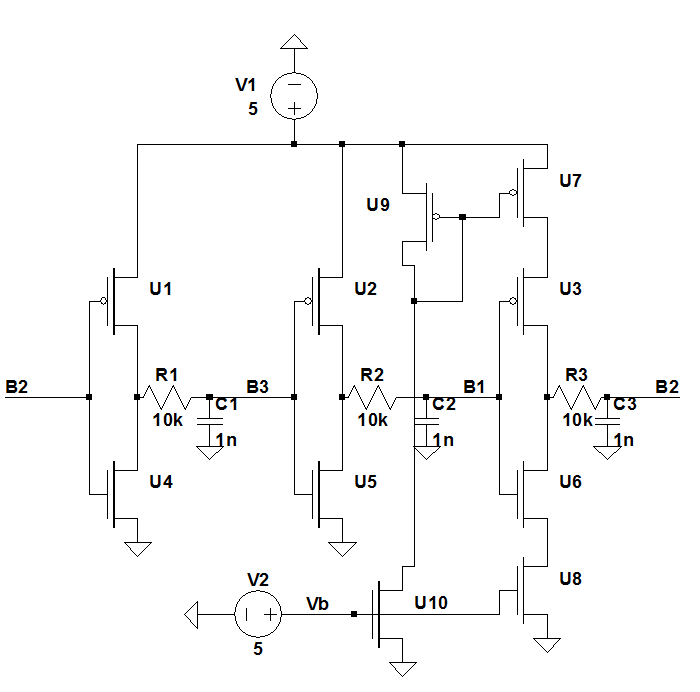
\includegraphics[scale=.5]{finalSchem2.png}
\caption{The schematic we used to simulate the oscillator in LTSpice}
\label{schem}
\end{figure}

To get an initial analysis of the circuit, we simulated a ring oscillator using LTSpice. The schematic that we used is shown in figure \ref{schem}. The oscillor consists of 3 inverters, one of which is ``starved'' of current (labeled B2). The bias voltage determines the oscillation frequency by limiting the current to branch 2. This branch takes longer to charge the capacitor, which limits the frequency. This current-starved inverter sets the fundamental frequency of the oscillator. \\

The signal from the starved inverter is amplified through each stage. This can be seen in figure \ref{lowBiasSigSim}. The bias transistor is in weak-moderate inversion, so it limits the output of the starved inverter. The signal is amplified twice, until it is about rail-to-rail on branch 1. Figure \ref{highBiasSigSim} shows that when the bias transistor is in strong inversion, the gain isn't very high. Note that for both cases, the branches are out of phase with each other. This is because as one inverter output is high, the other two are either rising or falling. \\


\begin{figure}[H]
\centering
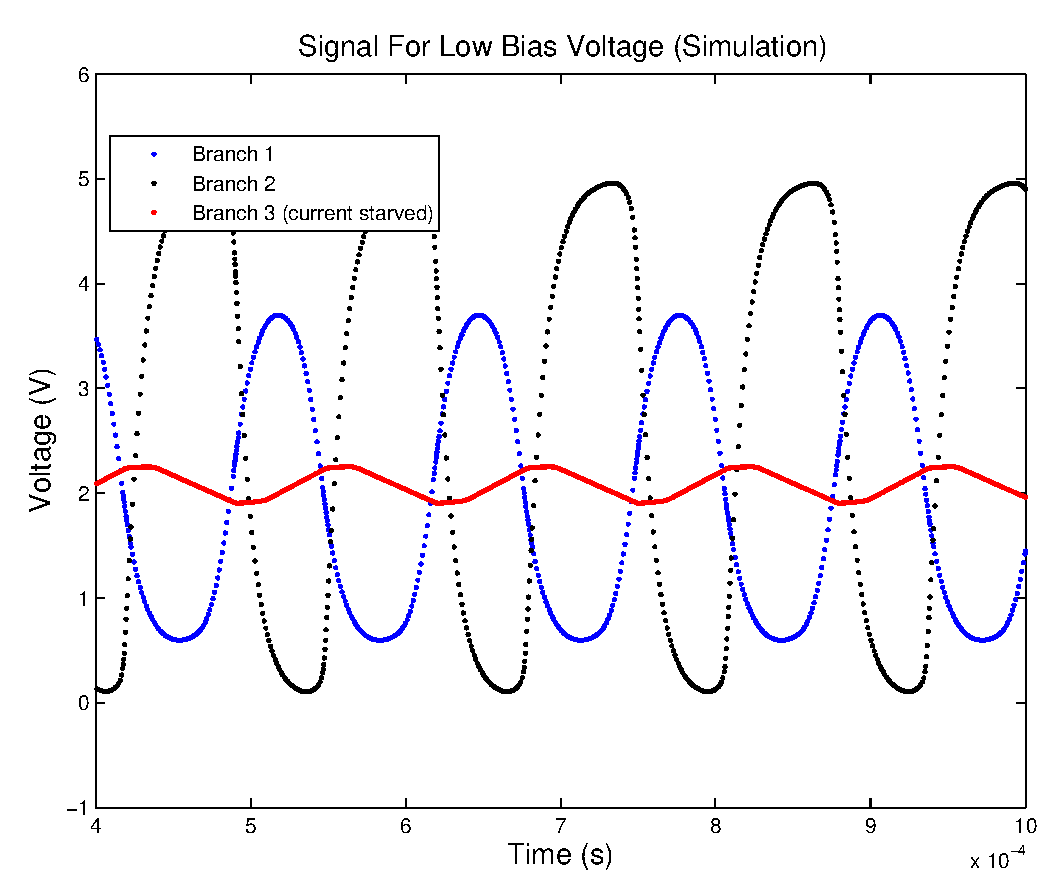
\includegraphics[scale=.7]{lowBiasSigSim.eps}
\caption{The output of each inverter for a low bias voltage.}
\label{lowBiasSigSim}
\end{figure}

\begin{figure}[H]
\centering
\includegraphics[scale=.7]{highBiasSigSim.eps}
\caption{The output of each inverter for a high bias voltage.}
\label{highBiasSigSim}
\end{figure}

Figure \ref{branch2DiffBiasSim} shows the differences in frequency between bias voltages. When the bias voltage is in moderate inversion, the current through the starved inverter is limited. Any change of bias voltage in this region causes a significant change in frequency. We found the frequency by calculating the period of each signal in MATLAB. We then plotted frequency as a function of bias voltage, which is shown in figure \ref{biasFrequenciesSim}. Note that for strong inversion, a change in the bias voltage has a relatively small effect on the frequency. 

\begin{figure}[H]
\centering
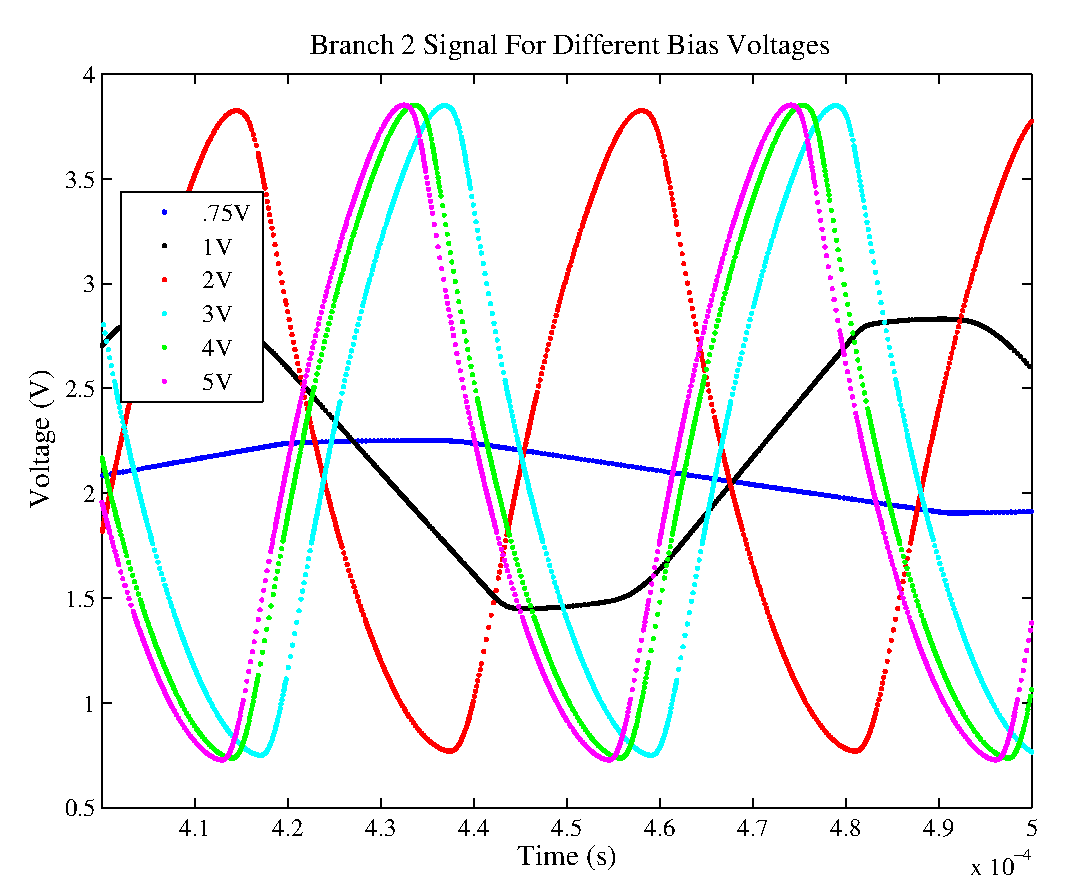
\includegraphics[scale=.7]{branch2DiffBiasSim.eps}
\caption{The output of the oscillator For different bias voltages. Note that increasing the bias voltage increases the frequency of the oscillator.}
\label{branch2DiffBiasSim}
\end{figure}


\begin{figure}[H]
\centering
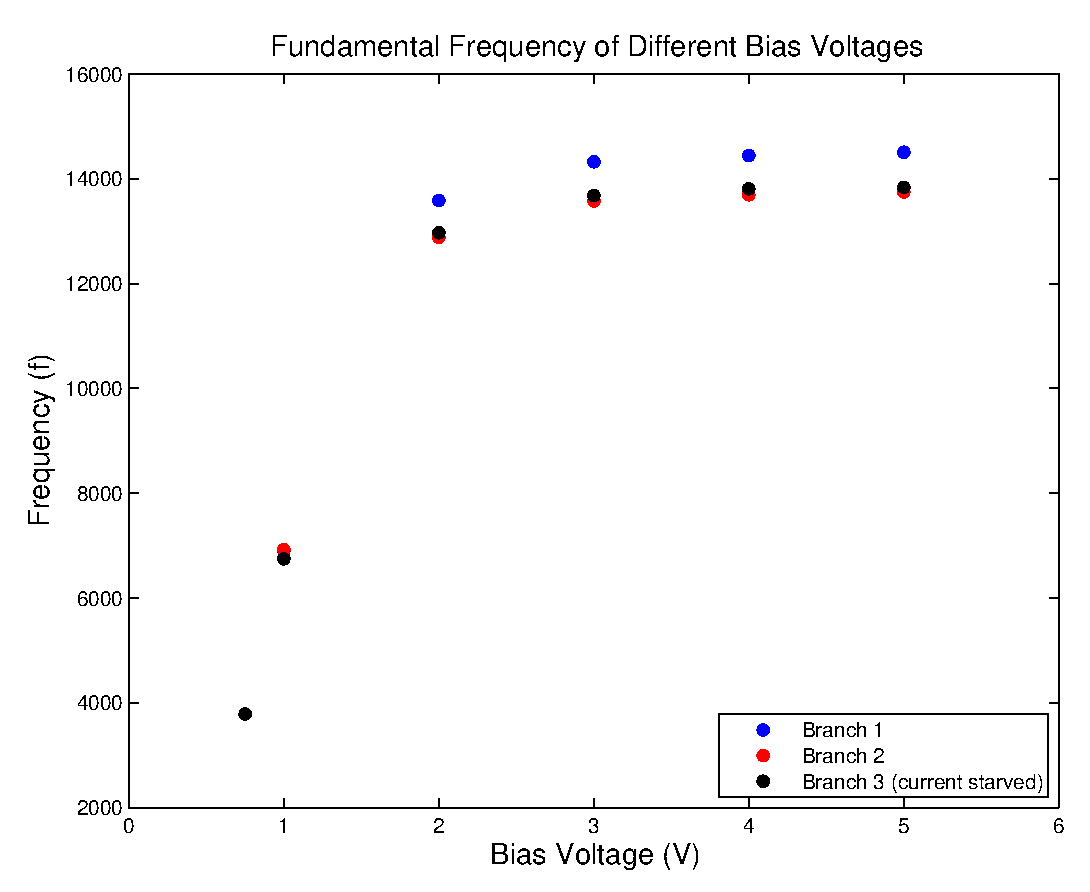
\includegraphics[scale=.7]{biasFrequenciesSim.eps}
\caption{The output frequency as a function of bias voltage. For a moderately inverted bias transistor, a change in bias voltage results in a large change in frequency.}
\label{biasFrequenciesSim}
\end{figure}

\section{Results}
talk about plots. maybe fit a theoretical to them.
plots:\\
signal for several bias voltages (same plot?)\\
signal for different branches\\
comparison to simulation results\\
frequency as a function of bias voltage\
\section{Postlab}
talk about stuff we didn't expect. why was one branch different? why do we exist? why driving a speaker doesn't make sense. Applications of our work. Which branch is the best if you are gonna make an oscillator? what should you do if you want frequencies above/below this range?

\end{document}